\documentclass{article}\usepackage[]{graphicx}\usepackage[]{xcolor}
% maxwidth is the original width if it is less than linewidth
% otherwise use linewidth (to make sure the graphics do not exceed the margin)
\makeatletter
\def\maxwidth{ %
  \ifdim\Gin@nat@width>\linewidth
    \linewidth
  \else
    \Gin@nat@width
  \fi
}
\makeatother

\definecolor{fgcolor}{rgb}{0.345, 0.345, 0.345}
\newcommand{\hlnum}[1]{\textcolor[rgb]{0.686,0.059,0.569}{#1}}%
\newcommand{\hlsng}[1]{\textcolor[rgb]{0.192,0.494,0.8}{#1}}%
\newcommand{\hlcom}[1]{\textcolor[rgb]{0.678,0.584,0.686}{\textit{#1}}}%
\newcommand{\hlopt}[1]{\textcolor[rgb]{0,0,0}{#1}}%
\newcommand{\hldef}[1]{\textcolor[rgb]{0.345,0.345,0.345}{#1}}%
\newcommand{\hlkwa}[1]{\textcolor[rgb]{0.161,0.373,0.58}{\textbf{#1}}}%
\newcommand{\hlkwb}[1]{\textcolor[rgb]{0.69,0.353,0.396}{#1}}%
\newcommand{\hlkwc}[1]{\textcolor[rgb]{0.333,0.667,0.333}{#1}}%
\newcommand{\hlkwd}[1]{\textcolor[rgb]{0.737,0.353,0.396}{\textbf{#1}}}%
\let\hlipl\hlkwb

\usepackage{framed}
\makeatletter
\newenvironment{kframe}{%
 \def\at@end@of@kframe{}%
 \ifinner\ifhmode%
  \def\at@end@of@kframe{\end{minipage}}%
  \begin{minipage}{\columnwidth}%
 \fi\fi%
 \def\FrameCommand##1{\hskip\@totalleftmargin \hskip-\fboxsep
 \colorbox{shadecolor}{##1}\hskip-\fboxsep
     % There is no \\@totalrightmargin, so:
     \hskip-\linewidth \hskip-\@totalleftmargin \hskip\columnwidth}%
 \MakeFramed {\advance\hsize-\width
   \@totalleftmargin\z@ \linewidth\hsize
   \@setminipage}}%
 {\par\unskip\endMakeFramed%
 \at@end@of@kframe}
\makeatother

\definecolor{shadecolor}{rgb}{.97, .97, .97}
\definecolor{messagecolor}{rgb}{0, 0, 0}
\definecolor{warningcolor}{rgb}{1, 0, 1}
\definecolor{errorcolor}{rgb}{1, 0, 0}
\newenvironment{knitrout}{}{} % an empty environment to be redefined in TeX

\usepackage{alltt}
\usepackage{amsmath} %This allows me to use the align functionality.
                     %If you find yourself trying to replicate
                     %something you found online, ensure you're
                     %loading the necessary packages!
\usepackage{amsfonts}%Math font
\usepackage{graphicx}%For including graphics
\usepackage{hyperref}%For Hyperlinks
\usepackage[shortlabels]{enumitem}% For enumerated lists with labels specified
                                  % We had to run tlmgr_install("enumitem") in R
\hypersetup{colorlinks = true,citecolor=black} %set citations to have black (not green) color
\usepackage{natbib}        %For the bibliography
\setlength{\bibsep}{0pt plus 0.3ex}
\bibliographystyle{apalike}%For the bibliography
\usepackage[margin=0.50in]{geometry}
\usepackage{float}
\usepackage{multicol}

%fix for figures
\usepackage{caption}
\newenvironment{Figure}
  {\par\medskip\noindent\minipage{\linewidth}}
  {\endminipage\par\medskip}
\IfFileExists{upquote.sty}{\usepackage{upquote}}{}
\begin{document}

\vspace{-1in}
\title{Lab 10 -- MATH 240 -- Computational Statistics}

\author{
  Caroline Devine \\
  Colgate University  \\
  Mathematics Department  \\
  {\tt cdevine@colgate.edu}
}

\date{04/08/2025}

\maketitle

\begin{multicols}{2}
%\raggedcolumns % If your spacing gets messed up try uncommenting 
                % this line
\begin{abstract}
This document provides a basic template for the 2-page labs we will complete each week. Here, briefly summarize what you did and why it might be helpful. Provide all the top-line conclusions, but avoid providing \emph{all} the details. Results should be limited to ``we show X, Y, and Z."
\end{abstract}

\noindent \textbf{Keywords:} What topics does the lab cover concerning class? List 3-4 key terms here, separated by semicolons.

\section{Introduction}

Gallup published a document called \emph{``How are Polls Conducted?"}. It outlines how Gallup selects people to include in its poll as well as other details. Focusing on two excerpts describing sample sizes of 1,000 and then 2,000, Gallup highlights how the results are accurate within a certain margin of error (\(\pm 4\% \) for n = 1000 and \(\pm 2\% \) for n = 2000). This margin of error tells researchers how much they can expect the sample proportion to differentiate from the proportion for the entire population. The goal of statisticians and quantitative researchers is to report a margin of error that provides 95\% confidence meaning they are 95\% confident that if they were to conduct the poll repeatably, they would contain the actual proportion 95\% of the time on the interval. The goal of this lab is to explore how sample size affects the margin of error as well as how to estimate this accurately. 

\section{Methods}
We will explore different simulations of different sample sizes and look at the differences in margins of errors through various mediums. To do this, we will look at basic simulation, resampling, simulations over different sample sizes and proportions, and calculate the actual margin of error. 

\subsection{Part 1: Basic Simulations}
Initially, we conducted a basic simulation study assuming a true probability that someone is satisfied with the position of United States in the world today to use the binomal distribution which measures the number of successes in a fixed number of trials. This was done using \texttt{rbinom()} function in \texttt{R}. We started with a sample size of 1,004 to replicate Gallup's example and doubled it for the second simulation completed. The sample proportion of the satisfied participants for each simulated poll was computed and plotted to visualize the distribution for both simulations. We also estimated the margin of error through calculation of the range of middle 95\% for comparison to Gallup's results. 

\subsection{Part 2: Resampling}

We assumed a true population proportion \emph{p} in part 1 which allowed us to see how the polls look like under that assumption, but in reality, we do not always know the true population proportion. To remove this assumption, we preform resampling to approximate the sampling distribution of \(\hat{p}\) using the Gallup survey data. This data reported that 39\% of respondents were satisfied with the position of the US in the world today, 59\% were dissatisfied, and 2\% had no opinion. These were categorized into ``satisfied", ``unsatisfied", and ``no opinion" categories for analysis, with the focus on estimating the proportion of respondents who were ``satisfied". Using the same sample size (n = 1004), we preformed 1,000 resamples and plotted them on a histogram with a superimposed density curve for visualization purposes. Margin of error was also calculated for comparison. 

\subsection{Part 3: Simulation over n and p}

To further explore how sample size(n) and the true population proportion(p) affects the margin of error, we simulated 10,000 simulations of a combination of increasing sample sizes and proportions. This is similar to the simulations in part 1, but at a larger scale. For each case, we calculated the margin of error using half of the range between the 2.5th and 97.5th percentiles of the sampling distribution. Using \texttt{geom\_raster()} function in \texttt{R} which produces a heatmap, we plotted the margin of error estimates across different values of n and p to visually see how population proportion and sample size affects margin of error.

\subsection{Part 4: Actual Margin of Error Calculation}

Estimating the margin of error from simulations is strong, but we can also find the actual margin of error through derivations of the Central Limit Theorem to find the Wilson Estimate analytically. The Wilson Estimate is a weighted average between \(\hat{P} = \frac{X}{n}\) and \(\frac{1}{2}\) where the weights are n and \(Z^2\) respectively. This provides an approximation of the margin of error called the Wilson margin of error formula:
$$
z_{1 - \alpha/2} * \frac{ \sqrt{n \hat{p} (1 - \hat{p}) + \frac{z_{1 - \alpha/2}^2}{4}} }{n + z_{1 - \alpha/2}^2}
$$
We computed the Wilson margin of error using the same values from part 3 for n and p and calculated z to be 1.96 using the standard normal distribution for a 95\% confidence interval. The table of errors were plotted them using a heatmap for comparison purposes. We did not need to use simulations for this step.

%% CODE FOR PLOTTING IN RESULTS AND APPENDIX %%


\section{Results}
\subsection{Basic Simulations}
The basic simulation study's goal was to examine how different sample sizes affects the sampling distribution and thus, the margin of error. Figure \ref{plot1} shows the visual representation of the sampling distrbutions and their density curves. Both appear to be approximately symmetric and bell-shaped. For \texttt{n = 1004}, the distribution is a relatively normal distribution is centered around 0.39. For \texttt{n = 2008}, the distribution has less variability because the spread of the sample proportions is more concentrated. Table \ref{table.1} corresponds to the graphical conclusions showing the margin of error decreasing as sample size increasings, aligning with Gallup's reported margins of error for each sample size. 
% latex table generated in R 4.4.2 by xtable 1.8-4 package
% Tue Apr  8 11:07:13 2025
\begin{table}[H]
\centering
\begingroup\small
\begin{tabular}{rrr}
  \hline
Sample Size & Range of middle 95\% & Margin of Error \\ 
  \hline
1004.00 & 0.06 & 0.03 \\ 
  2008.00 & 0.04 & 0.02 \\ 
   \hline
\end{tabular}
\endgroup
\caption{Margin of Error by Sample Size} 
\label{Table 1}
\end{table}


Figure 1

\subsection{resample}
% latex table generated in R 4.4.2 by xtable 1.8-4 package
% Tue Apr  8 11:07:13 2025
\begin{table}[H]
\centering
\begingroup\small
\begin{tabular}{rrr}
  \hline
Sample Size & Range of middle 95\% & Margin of Error \\ 
  \hline
1004.00 & 0.06 & 0.03 \\ 
   \hline
\end{tabular}
\endgroup
\caption{Margin of Error with Resampling} 
\label{Table 2}
\end{table}

Figure 2

\subsection{simulations + wilson}
Figure 3

Tie together the Introduction -- where you introduce the problem at hand -- and the methods --  what you propose to do to answer the question. Present your data, the results of your analyses, and how each reported aspect contributes to answering the question. This section should include table(s), statistic(s), and graphical displays. Make sure to put the results in a sensible order and that each result contributes a logical and developed solution. It should not just be a list. Avoid being repetitive. 

\subsection{Results Subsection}
Subsections can be helpful for the Results section, too. This can be particularly helpful if you have different questions to answer. 


\section{Discussion}
 You should objectively evaluate the evidence you found in the data. Do not embellish or wish-terpet (my made-up phase for making an interpretation you, or the researcher, wants to be true without the data \emph{actually} supporting it). Connect your findings to the existing information you provided in the Introduction.

Finally, provide some concluding remarks that tie together the entire paper. Think of the last part of the results as abstract-like. Tell the reader what they just consumed -- what's the takeaway message?

%%%%%%%%%%%%%%%%%%%%%%%%%%%%%%%%%%%%%%%%%%%%%%%%%%%%%%%%%%%%%%%%%%%%%%%%%%%%%%%%
% Bibliography
%%%%%%%%%%%%%%%%%%%%%%%%%%%%%%%%%%%%%%%%%%%%%%%%%%%%%%%%%%%%%%%%%%%%%%%%%%%%%%%%
\vspace{2em}

\noindent\textbf{Bibliography:} Note that when you add citations to your bib.bib file \emph{and}
you cite them in your document, the bibliography section will automatically populate here.

\begin{tiny}
\bibliography{bib}
\end{tiny}
\end{multicols}

%%%%%%%%%%%%%%%%%%%%%%%%%%%%%%%%%%%%%%%%%%%%%%%%%%%%%%%%%%%%%%%%%%%%%%%%%%%%%%%%
% Appendix
%%%%%%%%%%%%%%%%%%%%%%%%%%%%%%%%%%%%%%%%%%%%%%%%%%%%%%%%%%%%%%%%%%%%%%%%%%%%%%%%
\newpage
\onecolumn
\section{Appendix}


\begin{figure}[H]
\begin{center}
\begin{knitrout}
\definecolor{shadecolor}{rgb}{0.969, 0.969, 0.969}\color{fgcolor}

{\centering 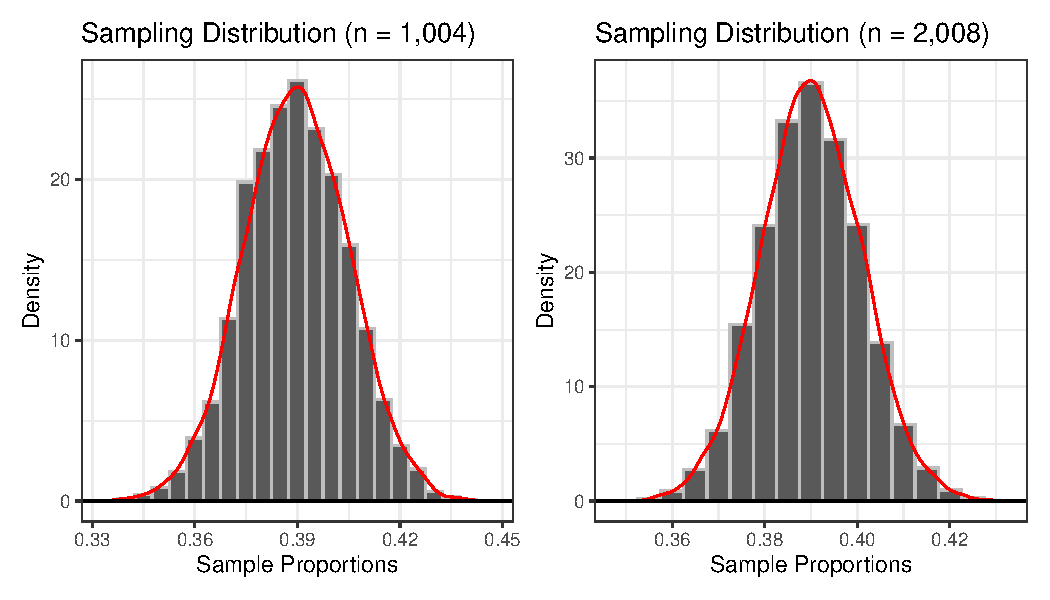
\includegraphics[width=\maxwidth]{figure/unnamed-chunk-4-1} 

}


\end{knitrout}
\caption{Sampling Distributions}
\label{plot1} 
\end{center}
\end{figure}


\begin{figure}[H]
\begin{center}
\begin{knitrout}
\definecolor{shadecolor}{rgb}{0.969, 0.969, 0.969}\color{fgcolor}

{\centering 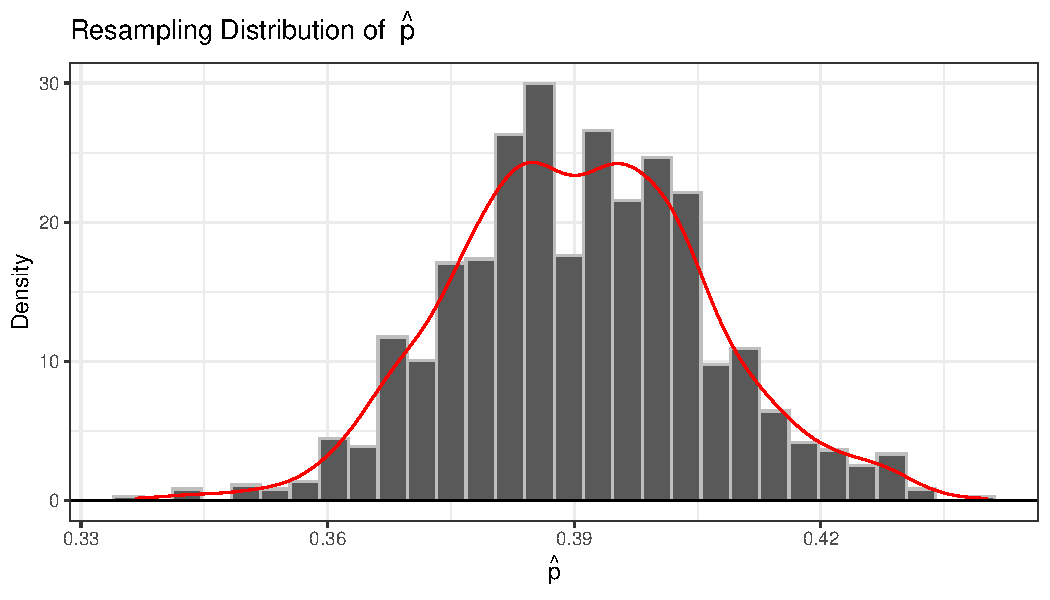
\includegraphics[width=\maxwidth]{figure/unnamed-chunk-5-1} 

}


\end{knitrout}
\caption{Resampling Distributions}
\label{plot2} 
\end{center}
\end{figure}



\begin{figure}[H]
\begin{center}
\begin{knitrout}
\definecolor{shadecolor}{rgb}{0.969, 0.969, 0.969}\color{fgcolor}

{\centering 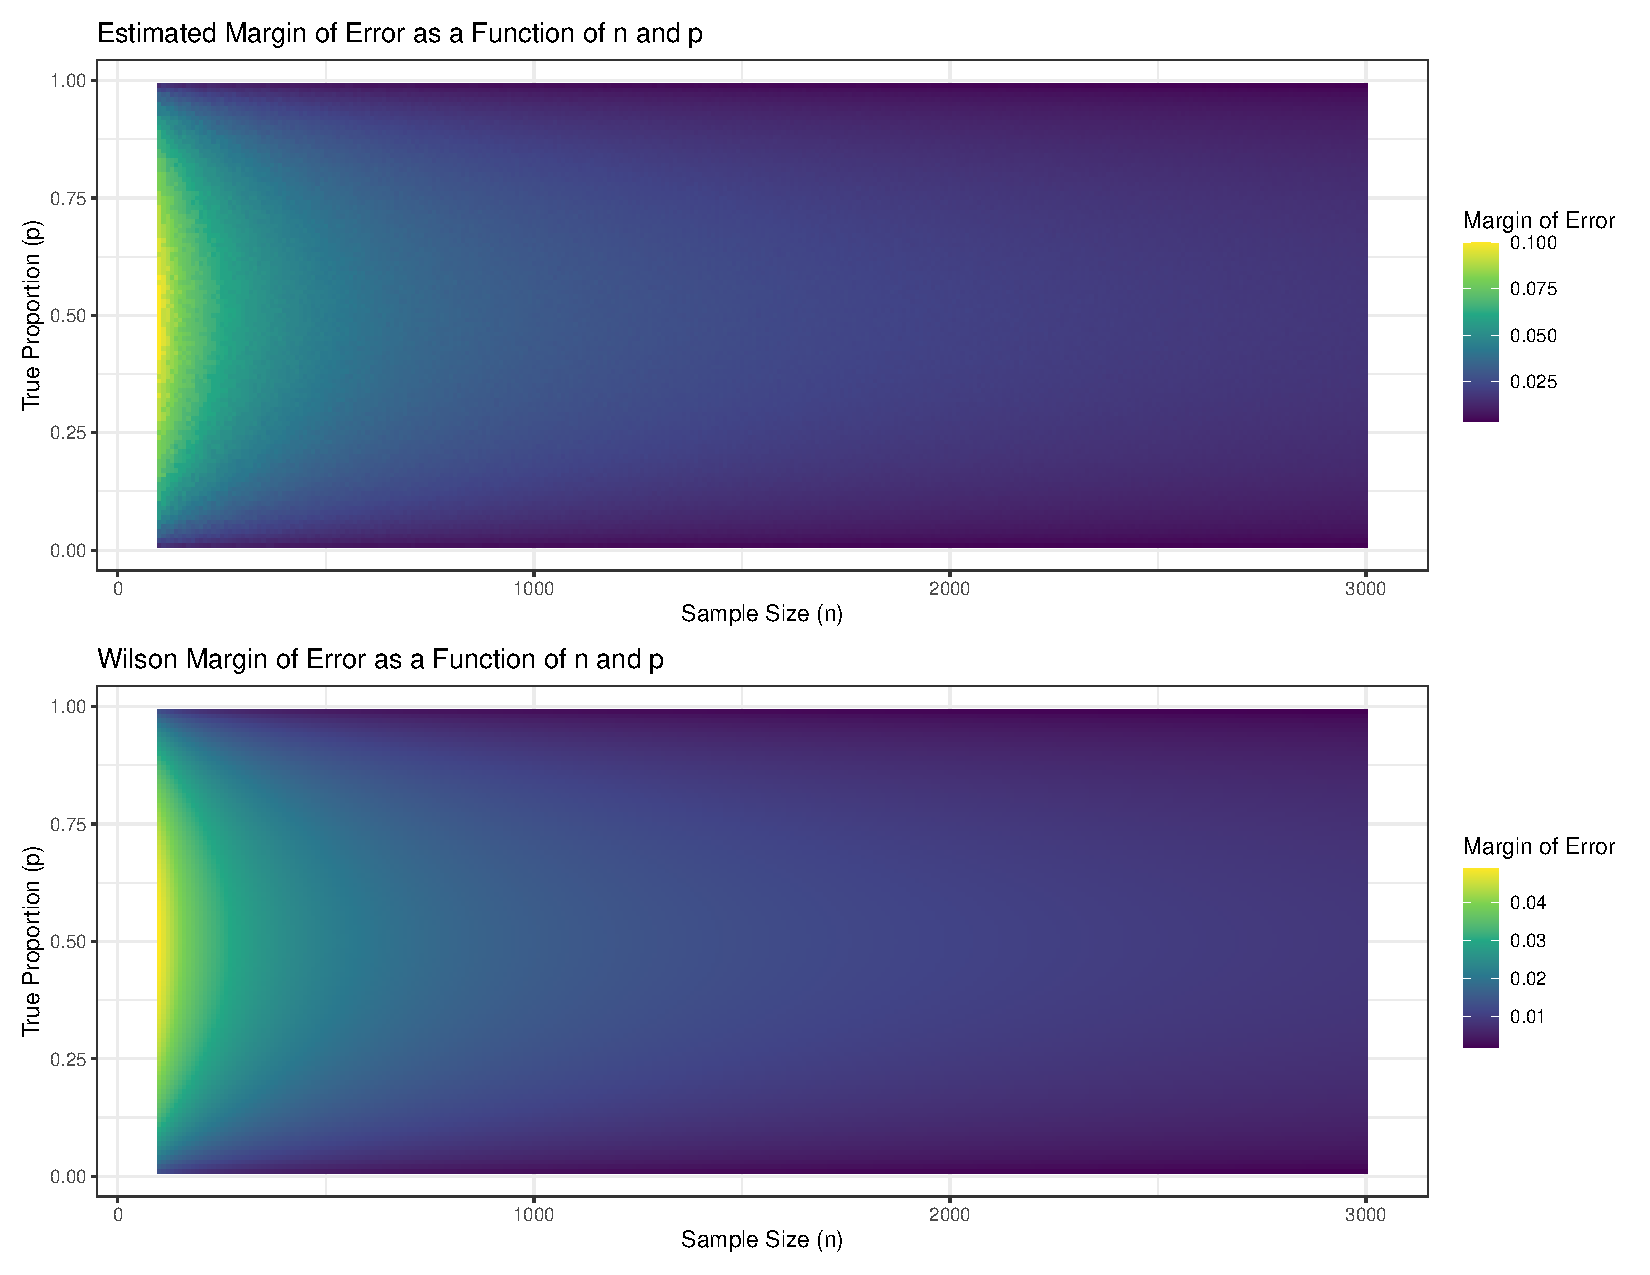
\includegraphics[width=\maxwidth]{figure/unnamed-chunk-6-1} 

}


\end{knitrout}
\caption{Heatmap: Margin of Error Comparisons}
\label{plot3} 
\end{center}
\end{figure}


\end{document}
